\documentclass[letter,11pt]{article}

\usepackage[spanish,es-nodecimaldot]{babel}
\usepackage[utf8]{inputenc}

\usepackage{lmodern}
\usepackage[T1]{fontenc}
\usepackage{textcomp}

\usepackage{framed}
\usepackage[svgnames]{xcolor}
\colorlet{shadecolor}{Gainsboro!50}

\usepackage{graphicx}
\usepackage{pstricks}

\usepackage{anysize}
\marginsize{3cm}{2cm}{2cm}{3cm}

\usepackage{amsmath}
\usepackage{array}
\usepackage{alltt}

\usepackage{fancyhdr}
\usepackage{lastpage}
\pagestyle{fancy}
\fancyhf{}
\fancyhead[LE,RO]{Laboratorio de Física Básica I}
\fancyfoot[CO,CE]{\thepage\ de \pageref{LastPage}}

\special{papersize=215.9mm,279.4mm}

\usepackage[
    pdfauthor={Carlos Eduardo Caballero Burgoa},%
    pdftitle={Laboratorio de Física Básica I},%
    pdfsubject={1er Parcial},%
    colorlinks,%
    citecolor=black,%
    filecolor=black,%
    linkcolor=black,%
    urlcolor=black,
    breaklinks]{hyperref}
\usepackage{breakurl}

\newcommand{\blankpage}{
\newpage
\thispagestyle{empty}
\mbox{}
\newpage
}

\renewcommand{\arraystretch}{1.2}

\begin{document}

\begin{center}
    {\Large \bf{Primer parcial}}
\end{center}

\noindent\fbox{%
    \parbox{\textwidth}{%
        Estudiante: CABALLERO BURGOA, Carlos Eduardo \\
        Carrera: Ingeniería Electromecánica \\
        Correo: cijkb.j@gmail.com
    }%
}

\vspace{1.0cm}

\begin{enumerate}
\item La tabla muestra una serie de medidas directas de la velocidad de un
    cuerpo en m/s. a) Exprese el resultado de la medición, su error absoluto y
    porcentual. b) La masa del cuerpo y su error es de:
    $m = (4.25\pm0.01)[kg]$. Calcule la energía cinética del cuerpo
    $E = \frac{1}{2}mv^2$, su error absoluto y porcentual utilizando el
    resultado del inciso anterior.

    \begin{center}
    \begin{tabular}{|c|c|c|c|c|c|c|c|c|}
    \hline
    No. & 1 & 2 & 3 & 4 & 5 & 6 & 7 & 8 \tabularnewline \hline
    $v[m/s]$ & 2.20 & 2.10 & 2.35 & 2.30 & 2.18 & 2.12 & 2.28 & 2.26 \tabularnewline \hline
    \end{tabular}
    \end{center}

    Solución: \\
    (a) \\

    \begin{tabular}{|c|>{\centering}m{3.2cm}<{\centering}
                      |>{\centering}m{2.8cm}<{\centering}
                      |>{\centering}m{4.0cm}<{\centering}|}
    \hline
    $i$ & $x_i$ & $x_i - \bar{x}$ & $(x_i - \bar{x})^2$ \tabularnewline \hline
      1 & 2.20 & -0.0237 & 0.0006 \tabularnewline \hline
      2 & 2.10 & -0.1237 & 0.0153 \tabularnewline \hline
      3 & 2.35 &  0.1263 & 0.0159 \tabularnewline \hline
      4 & 2.30 &  0.0762 & 0.0058 \tabularnewline \hline
      5 & 2.18 & -0.0437 & 0.0019 \tabularnewline \hline
      6 & 2.12 & -0.1037 & 0.0108 \tabularnewline \hline
      7 & 2.28 &  0.0562 & 0.0032 \tabularnewline \hline
      8 & 2.26 &  0.0362 & 0.0013 \tabularnewline \hline
    $n = 8$ & $\sum{x_i} = 17.79$ & & $\sum{(x_i - \bar{x})^2} = 0.0548$ \tabularnewline \hline
    \end{tabular}

    \begin{tabular}{|c|>{\centering}m{4.04cm}<{\centering}|}
    \hline
     $\bar{x}$ & 2.2237 \tabularnewline \hline
    $\sigma_x$ & 0.0313 \tabularnewline \hline
         $e_x$ & 0.0313 \tabularnewline \hline
    \end{tabular}

    \begin{tabular}{|c|>{\centering}m{7.52cm}<{\centering}|}
    \hline
    \multicolumn{2}{|c|}{\textbf{Velocidad}} \\ \hline
    $v$ & $(2.22\pm0.03)[m/s], 1.4\%$ \tabularnewline \hline
    \end{tabular}

    \vspace{1.0cm}
    \textbf{Memoria de calculo:}
    \begin{shaded}
        \begin{alltt}
            \footnotesize
\# Datos importados (i1.csv):
\input{resources/i1.csv}

\# Comandos ejecutados (p1a.m):
\input{resources/p1a.m}

\# Salida del programa (o1a.txt):
\input{resources/o1a.txt}
            \normalsize
        \end{alltt}
    \end{shaded}

    (b) \\
    \begin{center}
    \begin{tabular}{|c|>{\centering}m{5.0cm}<{\centering}|}
    \hline
    \multicolumn{2}{|c|}{\textbf{Medidas directas}}
    \tabularnewline \hline
    Velocidad ($v$) & $2.22 \pm 0.03 [m/s]; 1.4\%$
    \tabularnewline \hline
    Masa ($m$) & $4.25 \pm 0.01 [kg]; 0.40\%$
    \tabularnewline \hline
    \end{tabular}
    \end{center}

    \begin{equation*}
        E = \frac{1}{2} m v^2
    \end{equation*}

    Valor representativo:

    \begin{equation*}
        E = \frac{1}{2}(4.25)(2.22)^2 = 10.4729 [J]
    \end{equation*}

    Las derivadas parciales son:

    \begin{equation*}
        \frac{\partial{E}}{\partial{v}} = m v
    \end{equation*}
    \begin{equation*}
        \frac{\partial{E}}{\partial{m}} = \frac{1}{2} v^2
    \end{equation*}

    Siendo el error de la medición:

    \begin{equation*}
        e_V = \sqrt{
            \left(m v\right)^2{e_{v}}^2+
            \left(\frac{1}{2} v^2 \right)^2{e_{m}}^2
        }
    \end{equation*}

    Error representativo:

    \begin{equation*}
        e_V = \sqrt{
            \left((4.25)(2.22)\right)^2{0.03}^2+
            \left((0.5)(2.22)^2\right)^2{0.01}^2
        } = 0.2841
    \end{equation*}

    \begin{center}
    \begin{tabular}{|c|>{\centering}m{5.0cm}<{\centering}|}
    \hline
    \multicolumn{2}{|c|}{\textbf{Energía cinética}}
    \tabularnewline \hline
    Energía ($E$) & $(10.5 \pm 0.3)[J], 2.71\%$ \tabularnewline \hline
    \end{tabular}
    \end{center}

    \vspace{1.0cm}
    \textbf{Memoria de calculo:}
    \begin{shaded}
        \begin{alltt}
            \footnotesize
\# Comandos ejecutados (p1b.m):
\input{resources/p1b.m}

\# Salida del programa (o1b.txt):
\input{resources/o1b.txt}
            \normalsize
        \end{alltt}
    \end{shaded}

\newpage
\item La siguiente tabla es una relación funcional entre el periodo $T[s]$ y su
    longitud $L[m]$. a) Graficar $T = T(L)$. b) Linealicé aplicando logaritmos y
    graficar los datos logaritmizados. Obtenga a partir de la gráfica la
    ecuación del movimiento asumiendo un modelo potencial.

    \begin{center}
    \begin{tabular}{|c|>{\centering}m{2.8cm}<{\centering}
                      |>{\centering}m{2.8cm}<{\centering}|}
    \hline
    $i$ & $L_i [m]$ & $T_i [s]$ \tabularnewline \hline
      1 & 0.52 & 1.42 \tabularnewline \hline
      2 & 0.62 & 1.56 \tabularnewline \hline
      3 & 0.72 & 1.68 \tabularnewline \hline
      4 & 0.82 & 1.79 \tabularnewline \hline
      5 & 0.92 & 1.92 \tabularnewline \hline
      6 & 1.02 & 2.02 \tabularnewline \hline
    \end{tabular}
    \end{center}

    Solución: \\
    (a) \\

    Se obtiene el siguiente gráfico:

    \begin{figure}[!h]
    \centering
    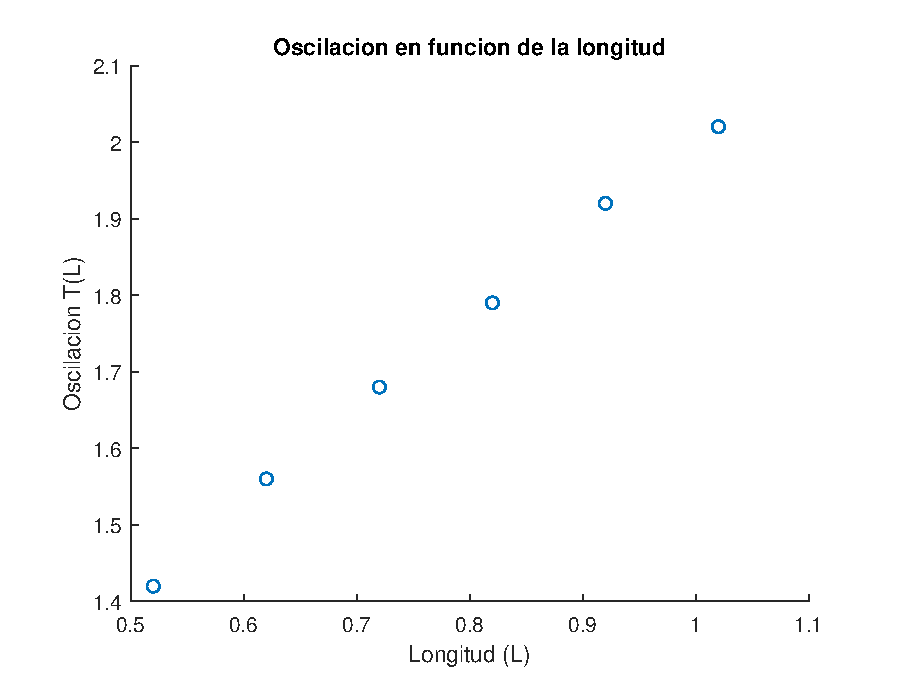
\includegraphics[scale=0.75]{resources/g2a.eps}
    \end{figure}

    (b) \\

    Aplicando linealización por logaritmos:

    La función tiene la forma general:

    \begin{equation*}
        y = a x^b
    \end{equation*}

    Aplicando logaritmos a ambos lados de la ecuación, obtenemos:

    \begin{equation*}
        \log y = \log a + b \log x
    \end{equation*}

    Haciendo los siguientes cambios de variables:

    \begin{equation*}
        Y' = \log y
    \end{equation*}
    \begin{equation*}
        A = \log a
    \end{equation*}
    \begin{equation*}
        B = b
    \end{equation*}
    \begin{equation*}
        X' = \log x
    \end{equation*}

    Se obtiene:

    \begin{equation*}
        Y' = A + B X'
    \end{equation*}

    \begin{center}
    \begin{tabular}{|c|>{\centering}m{2.8cm}<{\centering}
                      |>{\centering}m{2.8cm}<{\centering}|}
    \hline
    $i$ & $\log(L_i)$ & $\log(T_i)$ \tabularnewline \hline
      1 & -0.2840 & 0.1523 \tabularnewline \hline
      2 & -0.2076 & 0.1931 \tabularnewline \hline
      3 & -0.1427 & 0.2253 \tabularnewline \hline
      4 & -0.0862 & 0.2529 \tabularnewline \hline
      5 & -0.0362 & 0.2833 \tabularnewline \hline
      6 &  0.0086 & 0.3054 \tabularnewline \hline
    \end{tabular}
    \end{center}

    \begin{figure}[!h]
    \centering
    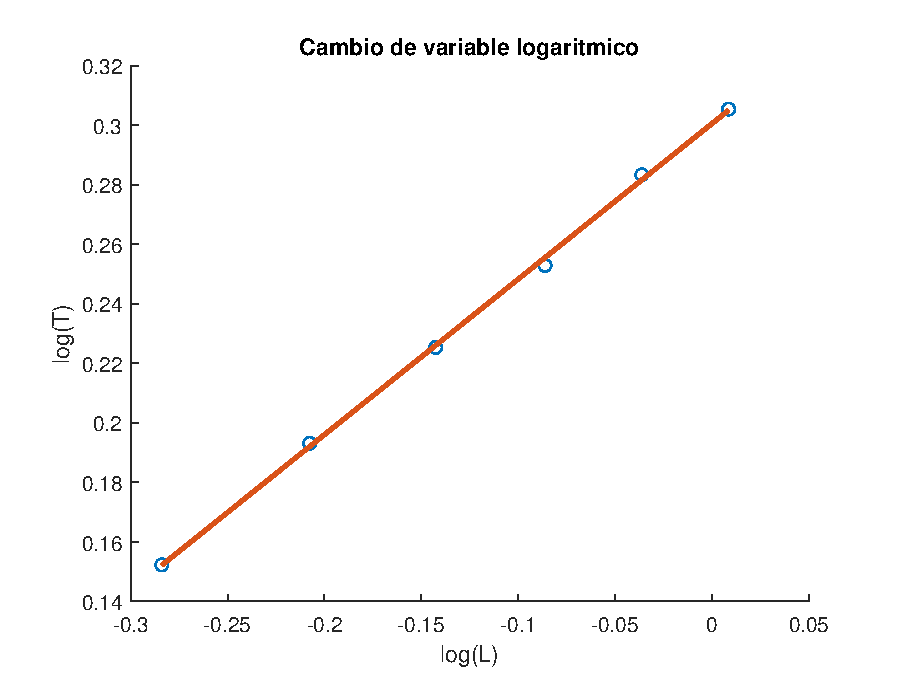
\includegraphics[scale=0.75]{resources/g2b.eps}
    \end{figure}

    \begin{equation*}
        B = \frac{0.3054-0.1523}{0.0086+0.2840} = \frac{0.1531}{0.2926} = 0.52
    \end{equation*}

    \begin{center}
    \begin{tabular}{|c|>{\centering}m{5.0cm}<{\centering}|}
    \hline
    \multicolumn{2}{|c|}{\textbf{Resultado}}
    \tabularnewline \hline
    $T$ & $a L^{0.5}$ \tabularnewline \hline
    \end{tabular}
    \end{center}

    \vspace{1.0cm}
    \textbf{Memoria de calculo:}
    \begin{shaded}
        \begin{alltt}
            \footnotesize
\# Datos importados (i2.csv):
\input{resources/i2.csv}

\# Comandos ejecutados (p2b.m):
\input{resources/p2b.m}

\# Salida del programa (o2b.txt):
\input{resources/o2b.txt}
            \normalsize
        \end{alltt}
    \end{shaded}

\newpage
\item La siguiente tabla es una relación funcional entre la presión $P[N/m^2]$ y
    el volumen $V [m^3]$ de un gas ideal; a) Obtenga la ecuación empírica
    mediante el método gráfico. b) A partir de los datos encuentre la ecuación
    empírica.

    \begin{center}
    \begin{tabular}{|c|>{\centering}m{2.8cm}<{\centering}
                      |>{\centering}m{2.8cm}<{\centering}|}
    \hline
    $i$ & $V_i [m^3]$ & $P_i [N/m^2]$ \tabularnewline \hline
      1 &  2.00 & 15.27 \tabularnewline \hline
      2 &  4.00 &  7.64 \tabularnewline \hline
      3 &  5.50 &  5.57 \tabularnewline \hline
      4 &  6.30 &  4.91 \tabularnewline \hline
      5 &  8.00 &  3.90 \tabularnewline \hline
      6 & 12.20 &  2.50 \tabularnewline \hline
    \end{tabular}
    \end{center}

    Solución: \\
    (a) \\

    Se obtiene el siguiente gráfico:

    \begin{figure}[!h]
    \centering
    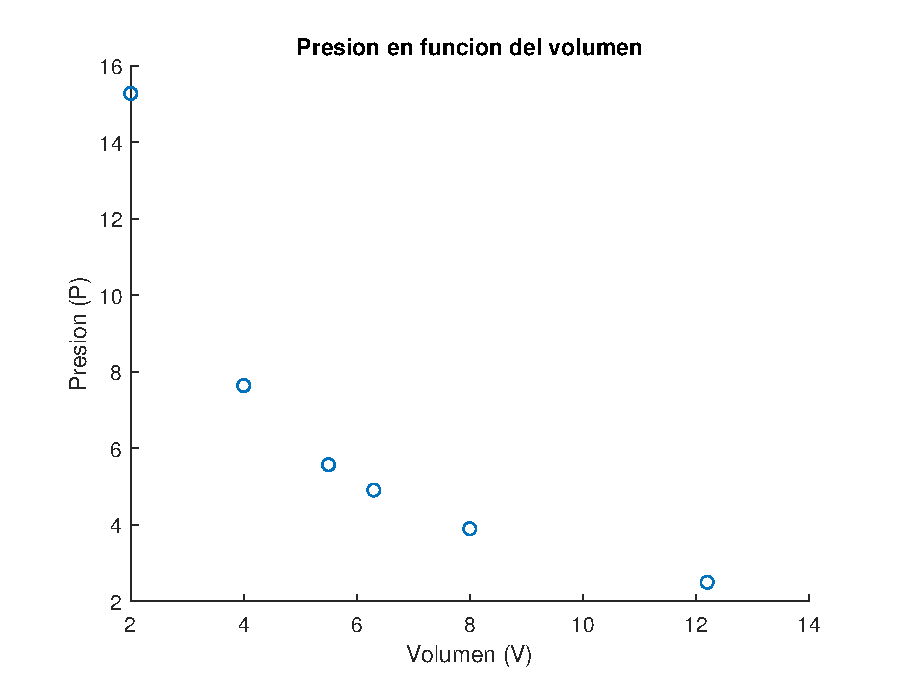
\includegraphics[scale=0.75]{resources/g3a.eps}
    \end{figure}

    Por tanto:

    \begin{equation*}
        P \propto \frac{1}{V}
    \end{equation*}

    \begin{center}
    \begin{tabular}{|c|>{\centering}m{5.0cm}<{\centering}|}
    \hline
    \multicolumn{2}{|c|}{\textbf{Resultado}}
    \tabularnewline \hline
    $P = \frac{A}{V}$ & Donde A es una constante \tabularnewline \hline
    \end{tabular}
    \end{center}

    (b) \\

    Aplicando linealización por logaritmos:

    La función tiene la forma general:

    \begin{equation}
        y = a x^b
    \end{equation}

    Aplicando logaritmos a ambos lados de la ecuación, obtenemos:

    \begin{equation*}
        \log y = \log a + b \log x
    \end{equation*}

    Haciendo los siguientes cambios de variables:

    \begin{equation*}
        Y' = \log y
    \end{equation*}
    \begin{equation*}
        A = \log a
    \end{equation*}
    \begin{equation*}
        B = b
    \end{equation*}
    \begin{equation*}
        X' = \log x
    \end{equation*}

    Se obtiene:

    \begin{equation*}
        Y' = A + B X'
    \end{equation*}

    \begin{center}
    \begin{tabular}{|c|>{\centering}m{2.8cm}<{\centering}
                      |>{\centering}m{2.8cm}<{\centering}|}
    \hline
    $i$ & $\log(V_i)$ & $\log(P_i)$ \tabularnewline \hline
      1 & 0.3010 & 1.1838 \tabularnewline \hline
      2 & 0.6021 & 0.8831 \tabularnewline \hline
      3 & 0.7404 & 0.7459 \tabularnewline \hline
      4 & 0.7993 & 0.6911 \tabularnewline \hline
      5 & 0.9031 & 0.5911 \tabularnewline \hline
      6 & 1.0864 & 0.3979 \tabularnewline \hline
    \end{tabular}
    \end{center}

    \begin{figure}[!h]
    \centering
    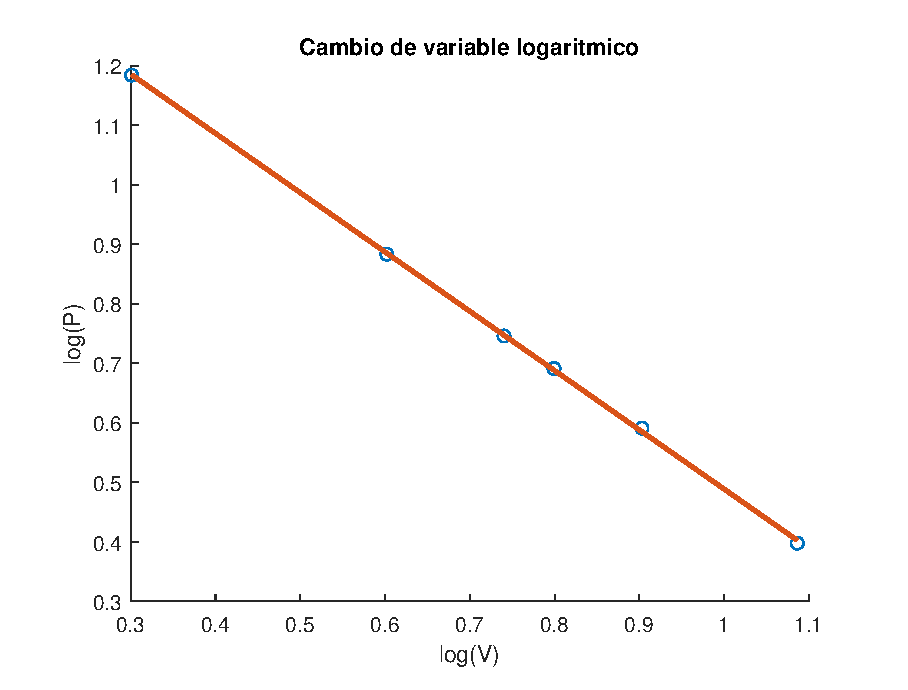
\includegraphics[scale=0.75]{resources/g3b.eps}
    \end{figure}

    \begin{equation*}
        B = \frac{0.3979-1.1838}{1.0864-0.3010} = \frac{-0.7859}{0.7854} = -1.00
    \end{equation*}

    \begin{center}
    \begin{tabular}{|c|>{\centering}m{5.0cm}<{\centering}|}
    \hline
    \multicolumn{2}{|c|}{\textbf{Resultado}}
    \tabularnewline \hline
    $P$ & $a V^{-1}$ \tabularnewline \hline
    \end{tabular}
    \end{center}

    \vspace{1.0cm}
    \textbf{Memoria de calculo:}
    \begin{shaded}
        \begin{alltt}
            \footnotesize
\# Datos importados (i3.csv):
\input{resources/i3.csv}

\# Comandos ejecutados (p3b.m):
\input{resources/p3b.m}

\# Salida del programa (o3b.txt):
\input{resources/o3b.txt}
            \normalsize
        \end{alltt}
    \end{shaded}

\newpage
\item La tabla presenta datos de masa $m$ y diámetro $D$ de esferas de un mismo
    material. a) Graficar $m = m(D)$, donde $m$ esta en $[g]$ y $D$ en $[cm]$
    b) Encuentre la ecuación empírica usando el método de cambio de variable y
    a partir de ella determine la densidad del material. Los datos fueron
    medidos con un tornillo micrométrico de $P = 0.001[cm]$ y la balanza digital
    de $P = 0.01[g]$.

    \begin{center}
    \begin{tabular}{|c|c|c|c|c|c|c|}
    \hline
    No. & 1 & 2 & 3 & 4 & 5 & 6 \tabularnewline \hline
    $D[cm]$ & 2.221 & 1.940 & 1.745 & 1.498 & 0.999 & 0.712 \tabularnewline \hline
    $m[g]$ & 44.75 & 28.20 & 21.71 & 13.75 & 4.09 & 1.48 \tabularnewline \hline
    \end{tabular}
    \end{center}

    Solución: \\
    (a) \\

    Se obtiene el siguiente gráfico:

    \begin{figure}[!h]
    \centering
    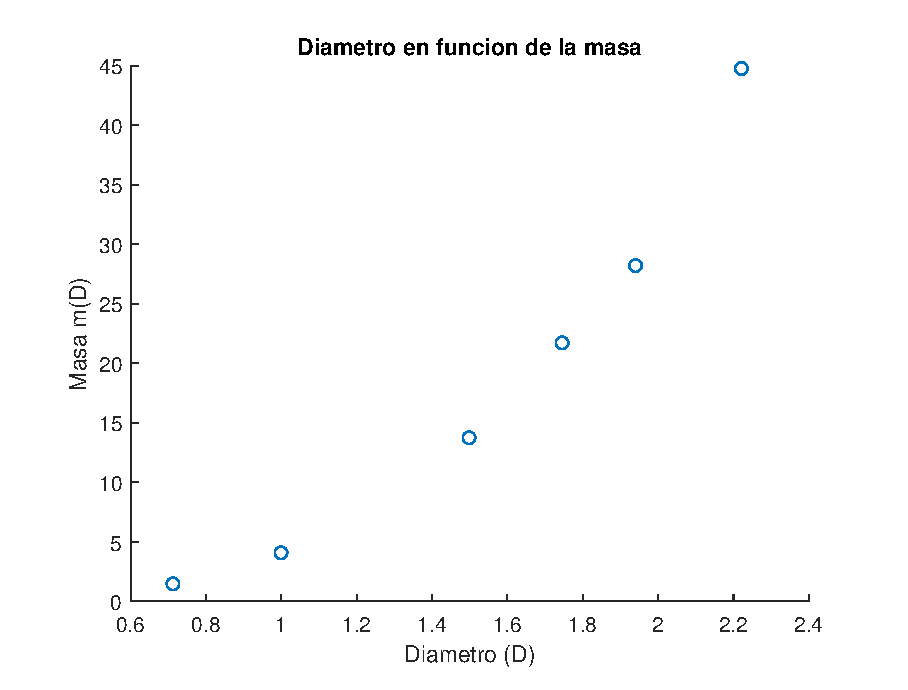
\includegraphics[scale=0.75]{resources/g4a.eps}
    \end{figure}

    (b) \\

    Aplicando cambio de variable:

    La función tiene la forma general:

    \begin{equation}
        y = a x^{3}
    \end{equation}

    Haciendo el siguiente cambio de variable:

    \begin{equation*}
        Z = x^{3}
    \end{equation*}

    Se obtiene:

    \begin{equation*}
        Y = A Z'
    \end{equation*}

    \begin{center}
    \begin{tabular}{|c|>{\centering}m{2.8cm}<{\centering}
                      |>{\centering}m{2.8cm}<{\centering}|}
    \hline
    $i$ & $D^3$ & $m$ \tabularnewline \hline
      1 & 10.9558 & 44.7500 \tabularnewline \hline
      2 &  7.3014 & 28.2000 \tabularnewline \hline
      3 &  5.3136 & 21.7100 \tabularnewline \hline
      4 &  3.3615 & 13.7500 \tabularnewline \hline
      5 &  0.9970 &  4.0900 \tabularnewline \hline
      6 &  0.3609 &  1.4800 \tabularnewline \hline
    \end{tabular}
    \end{center}

    \begin{figure}[!h]
    \centering
    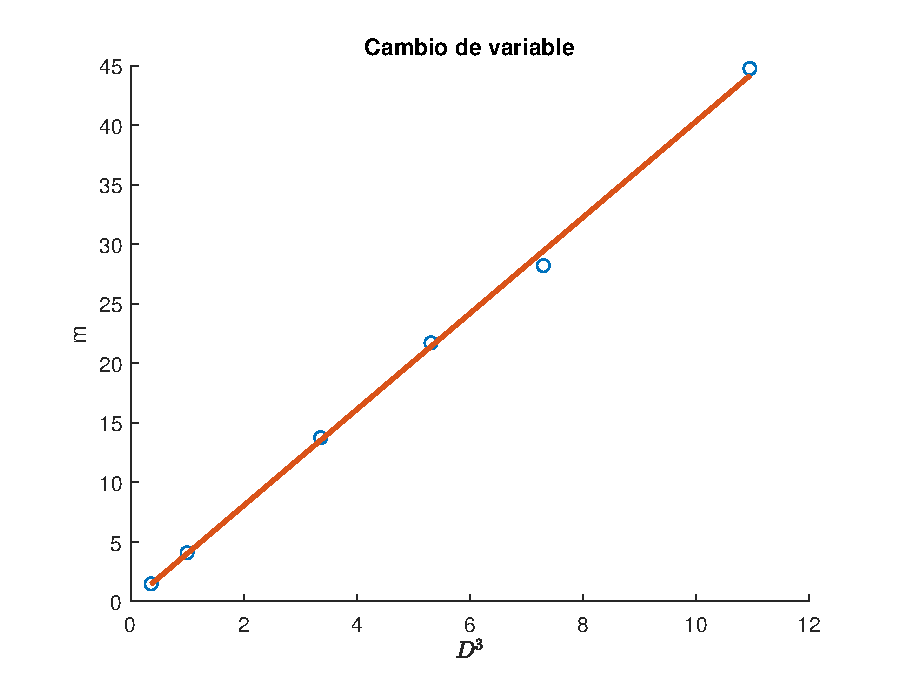
\includegraphics[scale=0.75]{resources/g4b.eps}
    \end{figure}

    \begin{equation*}
        B = \frac{1.4800-44.7500}{0.3609-10.9558} = \frac{-43.2700}{-10.5949} = 4.0840
    \end{equation*}

    \begin{center}
    \begin{tabular}{|c|>{\centering}m{5.0cm}<{\centering}|}
    \hline
    \multicolumn{2}{|c|}{\textbf{Resultado}}
    \tabularnewline \hline
    $m$ & $4.1 D^{3}$ \tabularnewline \hline
    \end{tabular}
    \end{center}

    \vspace{1.0cm}
    \textbf{Memoria de calculo:}
    \begin{shaded}
        \begin{alltt}
            \footnotesize
\# Datos importados (i4.csv):
\input{resources/i4.csv}

\# Comandos ejecutados (p4b.m):
\input{resources/p4b.m}

\# Salida del programa (o4b.txt):
\input{resources/o4b.txt}
            \normalsize
        \end{alltt}
    \end{shaded}

    Calculo de la densidad del material:

    Diametro:

    \begin{tabular}{|c|>{\centering}m{3.2cm}<{\centering}
                      |>{\centering}m{2.8cm}<{\centering}
                      |>{\centering}m{4.0cm}<{\centering}|}
    \hline
    $i$ & $x_i$ & $x_i - \bar{x}$ & $(x_i - \bar{x})^2$ \tabularnewline \hline
      1 & 2.2210 &  0.7018 & 0.4926 \tabularnewline \hline
      2 & 1.9400 &  0.4208 & 0.1771 \tabularnewline \hline
      3 & 1.7450 &  0.2258 & 0.0510 \tabularnewline \hline
      4 & 1.4980 & -0.0212 & 0.0004 \tabularnewline \hline
      5 & 0.9990 & -0.5202 & 0.2706 \tabularnewline \hline
      6 & 0.7120 & -0.8072 & 0.6515 \tabularnewline \hline
    $n = 6$ & $\sum{x_i} = 9.1150$ & & $\sum{(x_i - \bar{x})^2} = 1.6432$ \tabularnewline \hline
    \end{tabular}

    \begin{tabular}{|c|>{\centering}m{4.04cm}<{\centering}|}
    \hline
     $\bar{x}$ & 1.5192 \tabularnewline \hline
           $P$ & 0.001   \tabularnewline \hline
    $\sigma_x$ & 0.2340 \tabularnewline \hline
         $e_x$ & 0.2340 \tabularnewline \hline
    \end{tabular}

    \begin{tabular}{|c|>{\centering}m{7.52cm}<{\centering}|}
    \hline
    \multicolumn{2}{|c|}{\textbf{diametro}} \\ \hline
    $D$ & $(1.52\pm0.23)[m/s], 15.4\%$ \tabularnewline \hline
    \end{tabular}

    Masa:

    \begin{tabular}{|c|>{\centering}m{3.2cm}<{\centering}
                      |>{\centering}m{2.8cm}<{\centering}
                      |>{\centering}m{4.0cm}<{\centering}|}
    \hline
    $i$ & $x_i$ & $x_i - \bar{x}$ & $(x_i - \bar{x})^2$ \tabularnewline \hline
      1 & 44.7500 &  25.7533 & 663.2342 \tabularnewline \hline
      2 & 28.2000 &   9.2033 &  84.7013 \tabularnewline \hline
      3 & 21.7100 &   2.7133 &   7.3622 \tabularnewline \hline
      4 & 13.7500 &  -5.2467 &  27.5275 \tabularnewline \hline
      5 &  4.0900 & -14.9067 & 222.2087 \tabularnewline \hline
      6 &  1.4800 & -17.5167 & 306.8336 \tabularnewline \hline
    $n = 6$ & $\sum{x_i} = 113.98$ & & $\sum{(x_i - \bar{x})^2} = 1311.9$ \tabularnewline \hline
    \end{tabular}

    \begin{tabular}{|c|>{\centering}m{4.04cm}<{\centering}|}
    \hline
     $\bar{x}$ & 18.9967 \tabularnewline \hline
           $P$ & 0.01   \tabularnewline \hline
    $\sigma_x$ & 6.6128 \tabularnewline \hline
         $e_x$ & 6.6128 \tabularnewline \hline
    \end{tabular}

    \begin{tabular}{|c|>{\centering}m{7.52cm}<{\centering}|}
    \hline
    \multicolumn{2}{|c|}{\textbf{masa}} \\ \hline
    $m$ & $(19\pm6.6)[m/s], 34.81\%$ \tabularnewline \hline
    \end{tabular}

    \vspace{1.0cm}
    \textbf{Memoria de calculo:}
    \begin{shaded}
        \begin{alltt}
            \footnotesize
\# Datos importados (i4.csv):
\input{resources/i4.csv}

\# Comandos ejecutados (p4a.m):
\input{resources/p4bb.m}

\# Salida del programa (o4a.txt):
\input{resources/o4bb.txt}
            \normalsize
        \end{alltt}
    \end{shaded}

    \begin{equation*}
        \rho = \frac{m}{V} = \frac{3 m}{4 \pi r^2} = \frac{6m}{\pi D^3}
    \end{equation*}

    Valor representativo:

    \begin{equation*}
        \rho = \frac{6 (19)}{3.1415 (1.52)^3} = 10.35
    \end{equation*}

    Las derivadas parciales son:

    \begin{equation*}
        \frac{\partial{\rho}}{\partial{m}} = \frac{6}{\pi D^3}
    \end{equation*}
    \begin{equation*}
        \frac{\partial{\rho}}{\partial{D}} = -\frac{18 m}{\pi D^4}
    \end{equation*}

    Siendo el error de la medición:

    \begin{equation*}
        e_{\rho} = \sqrt{
            \left(\frac{6}{\pi D^3}\right)^2{e_{m}}^2+
            \left(-\frac{18 m}{\pi D^4}\right)^2{e_{D}}^2
        }
    \end{equation*}

    Error representativo:

    \begin{equation*}
        e_{\rho} = \sqrt{
            \left(0.5447\right)^2{6.61}^2+
            \left(-20.4334\right)^2{0.23}^2
        } = 5.9863
    \end{equation*}

    \begin{center}
    \begin{tabular}{|c|>{\centering}m{5.0cm}<{\centering}|}
    \hline
    \multicolumn{2}{|c|}{\textbf{Densidad}}
    \tabularnewline \hline
    Densidad ($\rho$) & $(10.35 \pm 5.98)[g/cm^3], 17.19\%$ \tabularnewline \hline
    \end{tabular}
    \end{center}

    \vspace{1.0cm}
    \textbf{Memoria de calculo:}
    \begin{shaded}
        \begin{alltt}
            \footnotesize
\# Comandos ejecutados (p4bbb.m):
\input{resources/p4bbb.m}

\# Salida del programa (o4bbb.txt):
\input{resources/o4bbb.txt}
            \normalsize
        \end{alltt}
    \end{shaded}

\end{enumerate}
\end{document}

